\clearpage
\section{Versuchsaufbau}
Der Versuchsaufbau besteht aus folgenden Komponenten:
\begin{itemize}
	\item Strahlungsquelle
	\item Halbleiterdetektor
	\item Vakuumgefäß mit Manometer, Ein- und Auslassventil
	\item Vakuumpumpe
	\item Vorverstärker und Hauptverstärker für die Detektorsignale
	\item Spannungsversorgungsgerät mit externem Spannungsmessgerät
	\item Vielkanalpulshöhenanalysator (Multi Channel Analysator -- MCA)\\im PC
	\item PC mit MCA-Software
\end{itemize}

Abbildung \ref{fig:aufbauhalbleiter} zeigt den Versuchsaufbau schematisch, Fotos sind in Abbildung \ref{fig:setup_} zu sehen. Der Oberflächensperrschichtzähler und die Alphastrahlungsquelle befinden sich in einem luftdichten Metallzylinder. Die Quelle lässt sich im Zylinder entlang einer Raumachse verschieben, um den Abstand zwischen Quelle und Detektor verändern zu können. Bei minimalem einstellbaren Abstand berühren sich Quelle und Detektor nicht, die Bestimmung dieses Nullabstandes ist Teil des Versuchs.
\begin{figure}[h]
	\centering
	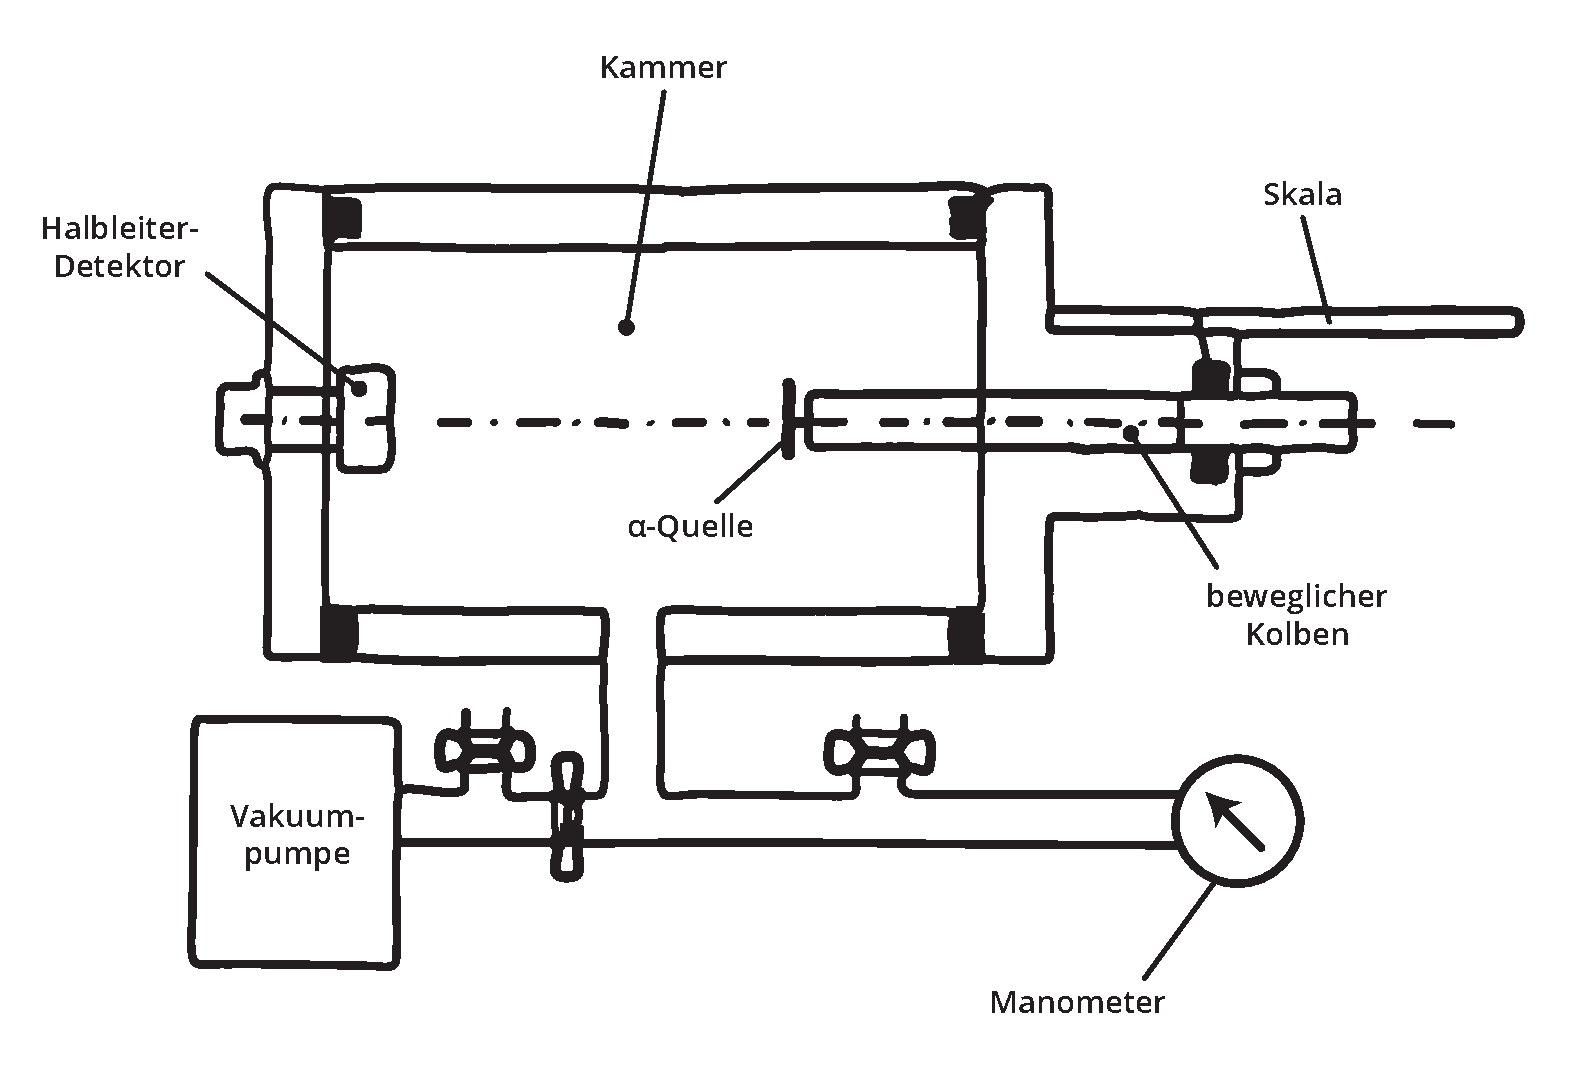
\includegraphics[width=0.7\linewidth]{img/aufbau_halbleiter}
	\caption{Versuchsaufbau}
	\label{fig:aufbauhalbleiter}
\end{figure}

Die Mischquelle hat einen aktiven Bereich mit einem Durchmesser von circa 7~mm und ist durch eine etwa 2~\textmu m dicke Goldschicht abgedeckt (siehe Abb. \ref{fig:quellefoto}). Die Abdeckung des radioaktiven Materials bietet bei Kontakt keinen Schutz vor Kontamination, deshalb muss die Quelle als offen angesehen werden. Für den Umgang mit offenen Quellen sind besondere Genehmigungsauflagen und Vorsichtsmaßnahmen zu beachten (siehe Abschnitt \ref{sec:warnhinweise}).

An den Halbleiterdetektor ist direkt außerhalb des Vakuumkolbens der Vorverstärker angebracht. Das Eintrittsfenster des Detektors ist in Abbildung \ref{fig:detektorfoto} zu sehen. Der Vorverstärker besitzt mehrere Anschlüsse: 
\begin{itemize}[itemsep=0pt]
	\item Versorgung Betriebsspannung, angeschlossen an der Rückseite des Hauptverstärkers. 
	\item Signalausgang, verbunden mit Signaleingang des Hauptverstärkers.
	\item Eingang externe Spannung, verbunden mit Spannungsversorgungsgerät.
	\item Anschlussmöglichkeit für einen Pulser. Nicht verbunden.
\end{itemize}
Die Verkabelung des Versuches ist in Abbildung \ref{fig:verkabelung} dargestellt und Abbildung \ref{fig:setup3} zeigt ein Foto des Hauptverstärkers sowie des Spannungsversorgungsgerätes.
%
\begin{figure}[h]
	\centering
	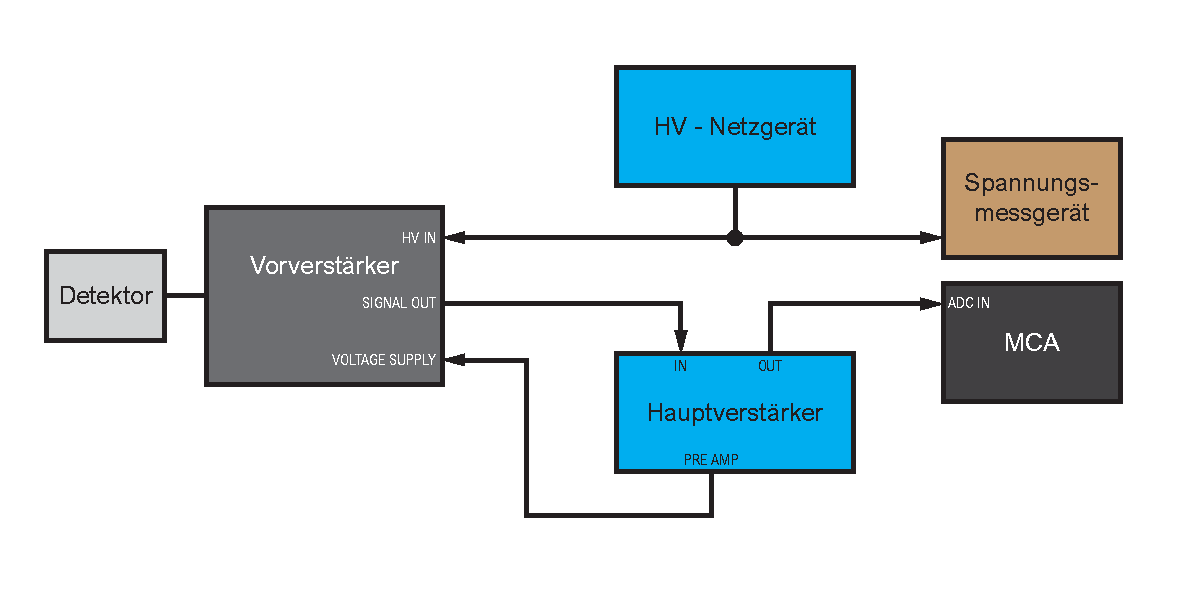
\includegraphics[width=\linewidth]{img/verkabelung}
	\caption{Schematische Darstellung der Verkabelung}
	\label{fig:verkabelung}
\end{figure}

\begin{figure}
	\centering
	\subcaptionbox{Ansicht von links. \label{fig:setup1}}[.49\linewidth]{\includegraphics[width=\linewidth]{img/setup_1.jpg}}
	\subcaptionbox{Ansicht von rechts. \label{fig:setup2}}[.49\linewidth]{\includegraphics[width=\linewidth]{img/setup_2.jpg}}
	\caption{Der Versuchsaufbau}
	\label{fig:setup_}
\end{figure}
\begin{figure}
	\centering
	\subcaptionbox{Der Halbleiterdetektor. \label{fig:detektorfoto}}[.49\linewidth]
	{\includegraphics[width=\linewidth]{img/detektor_foto}}
	\subcaptionbox{Die Mischquelle mit goldener Oberfläche. \label{fig:quellefoto}}[.49\linewidth]
	{\includegraphics[width=\linewidth]{img/quelle_foto}}
	\caption{Innenansichten des Vakuumgefäßes (Container).}
\end{figure}
\begin{figure}
	\centering
	\includegraphics[width=0.75\linewidth]{img/setup_3.jpg}
	\caption{Zugehörige Elektronik im \enquote{Ortec-Crate}.}
	\label{fig:setup3}
\end{figure}


